%\subsection{Perturbation}
\subsection{Differential Privacy}

Differential Privacy ist eine Technik, welche 2006 von Cynthia Dwork \cite{P-26} vorgestellt wurde.
Ziel dabei ist es, Zugriff auf einen Datensatz zu ermöglichen, der sowohl nützliche Erkenntnisse zulässt, als auch die Privatsphäre eines einzelnen Datenpunktes schützt.


Diese beiden Ziele sind laut Dwork \cite{P-26} erfüllt, wenn Anfragen auf zwei Datensätze, die sich in höchstens einem Datenpunkt unterscheiden, keine signifikanten Unterschiede aufweise. 
Um dies zu erreichen, wird den Anfragen ein zufälliges Rauschen hinzugefügt. 
Dadurch handelt es sich bei Abfragen um randomisierte Funktionen.
Die Größe des Unterschied der gleichen Abfrage auf zwei Datensätze, die sich in höchstens einem Eintrag unterscheiden, kann durch einen Wert $\epsilon$ dargestellt werden.

Formal lautet die Definition von $\epsilon$-Differential Privacy wie folgt \cite{P-26}:\\
\textit{
Eine randomisierte Funktion $M$, welche einen Datensatz $D$ auf einen Wertebereich $R$ abbildet, weist $\epsilon$-Differential Privacy auf, wenn für alle Datensätze $D_{1}$ und $D_{2}$ die sich in höchstens einem Datenpunkt unterscheiden, gilt:}
\begin{equation}
    Pr[M(D_{1}) \in R] \leq e^{\epsilon} \times Pr[\kappa(D_{2}) \in R]
\end{equation}

Dwork und Roth \cite{P-27} fügten der Definition noch einen Parameter $\delta$ hinzu, welcher erlaubt, dass die Voraussetzungen zu einem definierten Grad verletzt werden können.
Die damit angepasste Definition von ($\epsilon$,$\delta$)-Differential Privacy lautet \cite{P-27}:\\
%Damit lautet die formale Definition von Differential Privacy wie folgt \cite{P-27}:
\textit{
    Eine randomisierte Funktion $M$, welche einen Datensatz $D$ auf einen Wertebereich $R$ abbildet, erfüllt ($\epsilon$,$\delta$)-Differential Privacy, wenn für alle Datensätze $D_{1}$ und $D_{2}$, die sich in höchstens einem Datenpunkt unterscheiden, gilt:}
\begin{equation}
    Pr[M(D_{1}) \in R] \leq e^{\epsilon} \times Pr[M(D_{2}) \in R] + \delta
\end{equation} 

Konkret sagen die Definitionen aus, dass eine randomisierte Funktion, auf beiden Datensätzen angewendet, nahezu die gleichen Ergebnisse liefert. 
Dabei bestimmten $\epsilon$ und $\delta$ wie stark sich die Ergebnisse unterscheiden dürfen.

\begin{figure}[!htb]
    \centering
    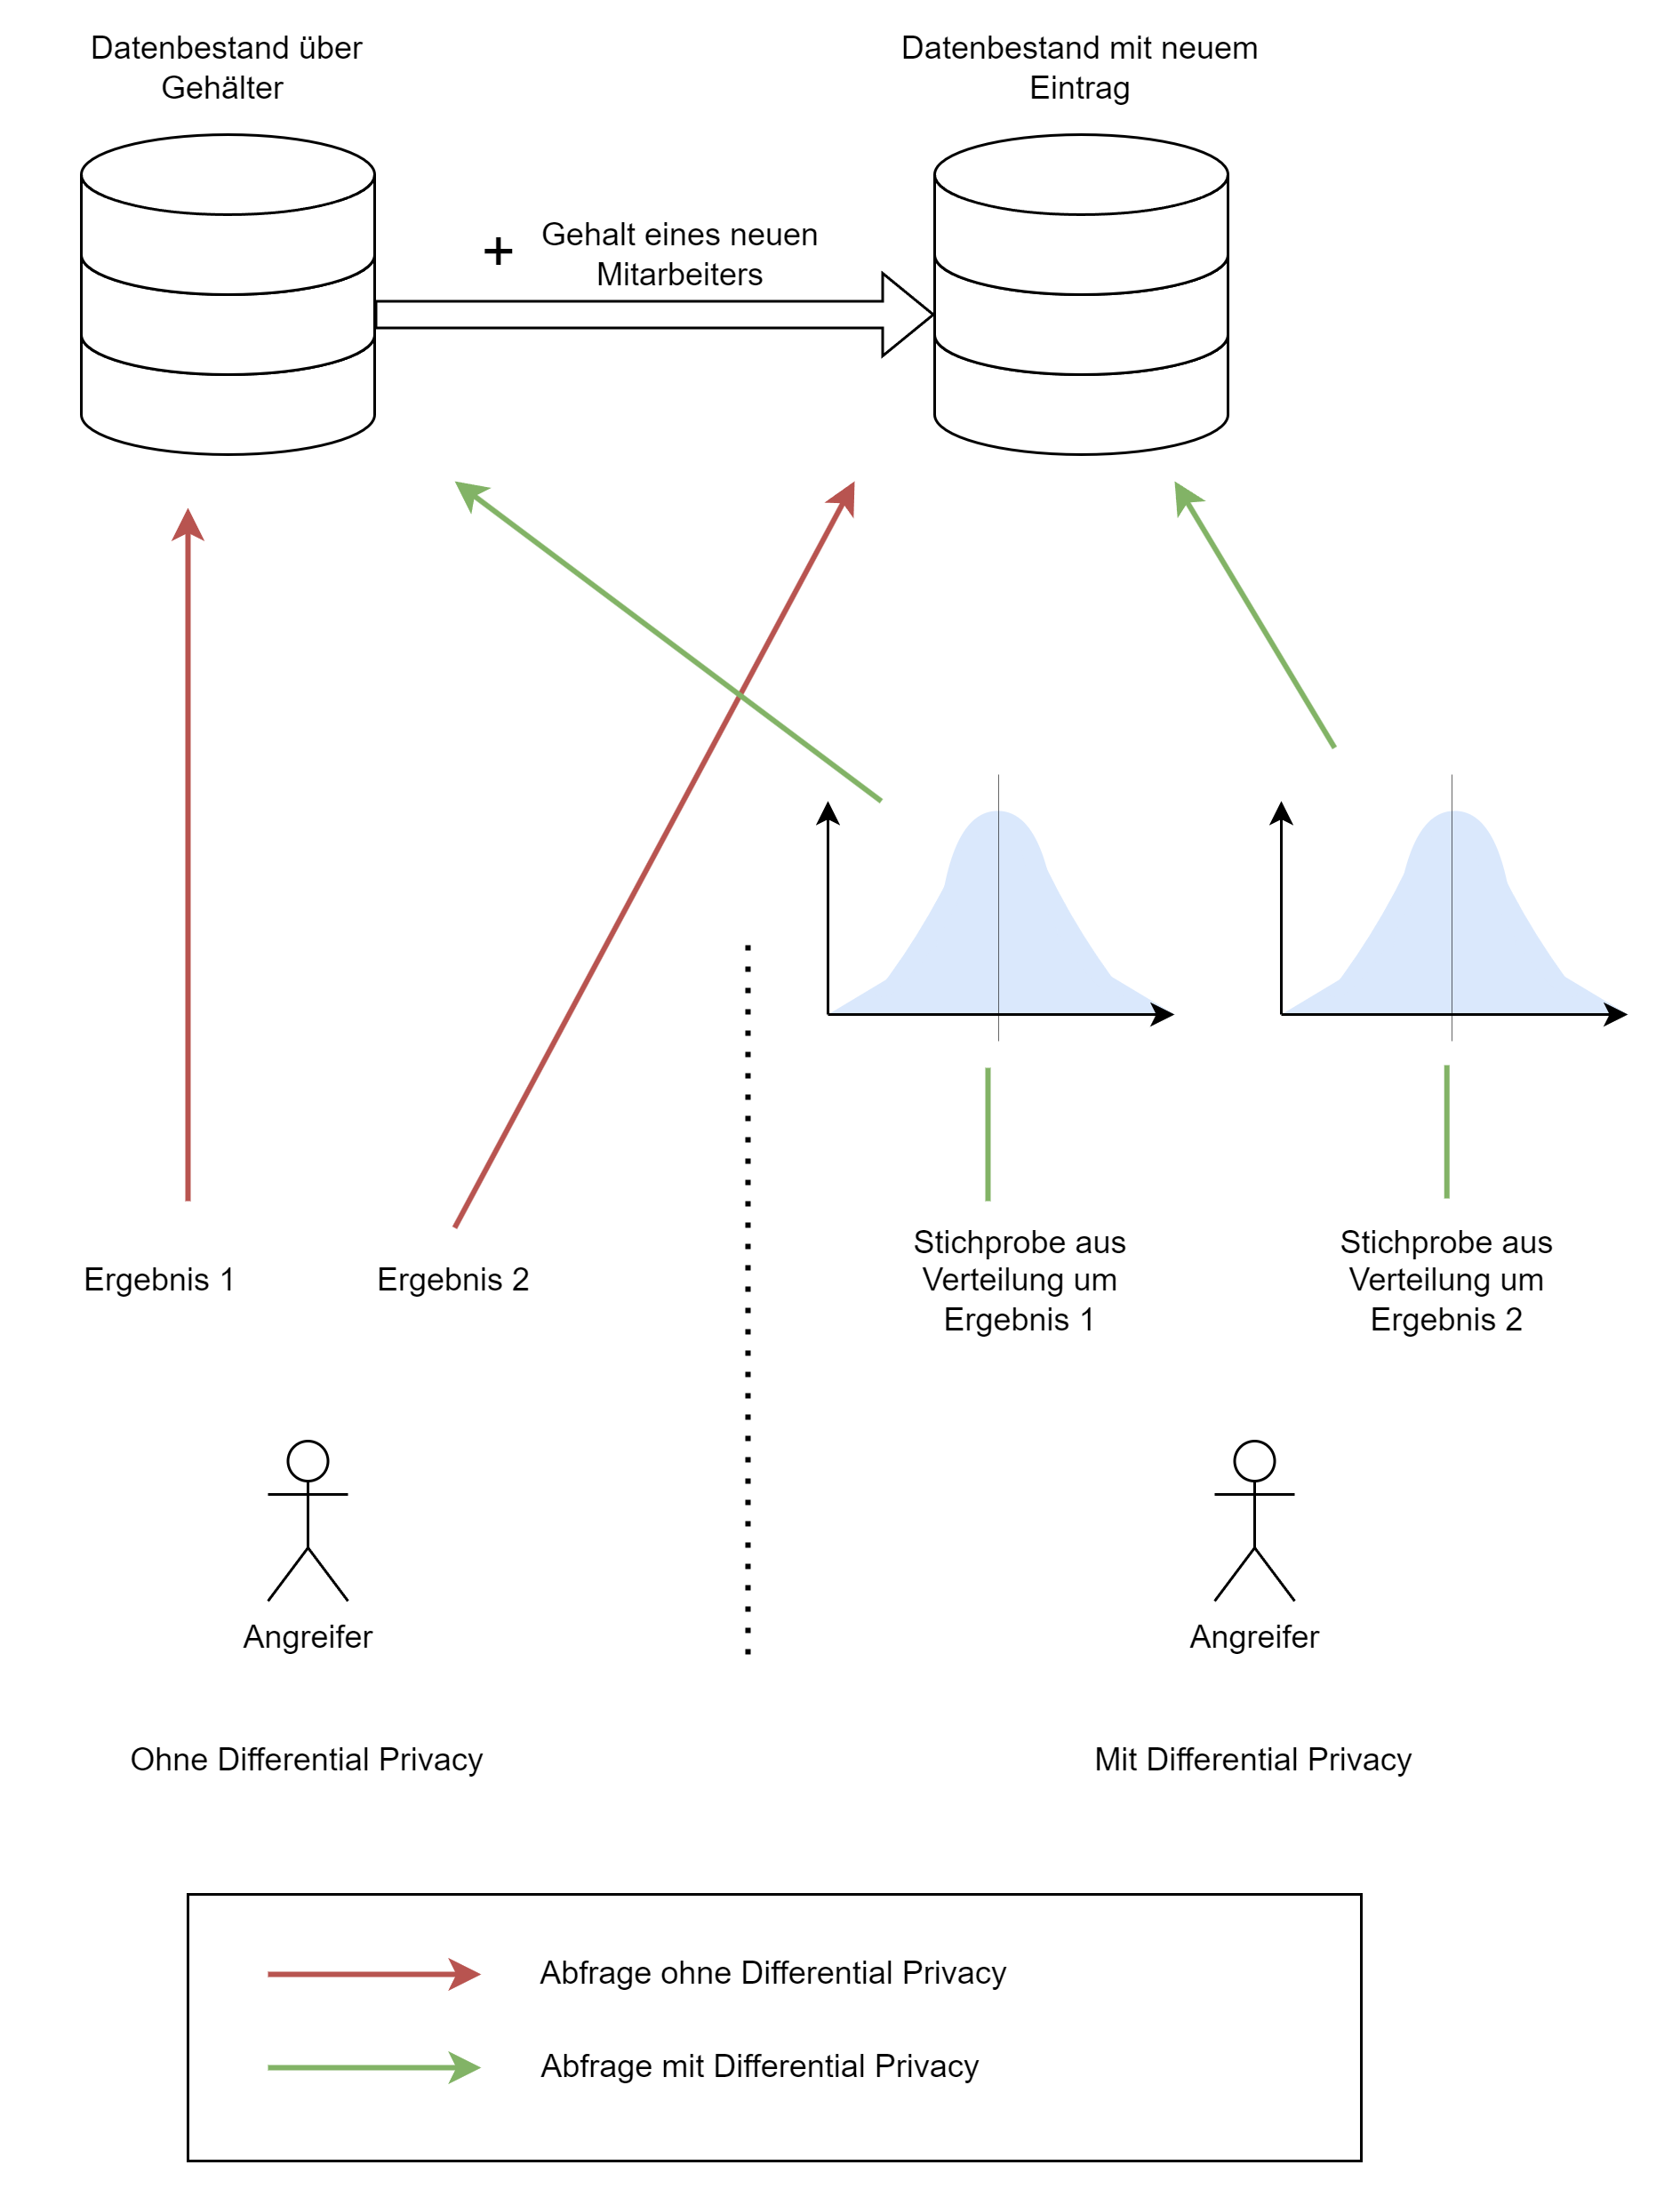
\includegraphics[width=10cm]{figures/dp}
    \caption{Beispiel Differential Privacy}
    \label{fig:dp}
\end{figure} 

Abbildung \ref{fig:dp} zeigt exemplarisch, wie Differential Privacy anhand einer Abfrage des Durchschnittsgehalts eines Unternehmens aussehen könnte.
Dabei führt ein Angreifer 2 Anfragen aus, auf die gleiche Datenbank, welche aber bei Anfrage 2 um einen zusätzlichen Gehaltseintrag eines neuen Mitarbeiters erweitert wurde.
Würde kein Differential Privacy genutzt werden, könnte anhand der Anzahl der Mitarbeiter und der beiden durchschnittlichen Gehältern das exakte Gehalt des neuen Mitarbeiters berechnet werden.
Wird nun Differential Privacy genutzt, wird ein zufälliges Rauschen über das Ergebnis der Anfrage gelegt, wodurch Anfrage 1 und 2 ein nahezu identisches Ergebnis ausliefern, abhängig der Parameter $\epsilon$ und $\delta$.

Differential Privacy kann dabei an 3 unterschiedlichen Stellen der Machine Learning Pipeline genutzt werden:
\begin{compactitem}
\item \textbf{Vorbereitung der Trainingsdaten:} Diese Methodik wird folgend in diesem Kapitel erläutert.
\item \textbf{Trainingsalgorithmus:} Kapitel \ref{sec:dp_training} beschreibt, welche Anpassung am Trainingsalgorithmus vorgenommen werden müssen, damit dieser Differential Privacy nutzen kann.
\item \textbf{Vorhersage des Modells:} Wie der Output des Modells durch Nutzung von Differential Privacy geschützt werden kann, wird durch Kapitel \ref{sec:dp_output} dargestellt.
\end{compactitem}


